% \documentclass[tikz, border=10pt]{standalone}
% cf http://cloford.com/resources/colours/websafe1.htm
\definecolor{sv-all}{RGB}{255,153,255}
\definecolor{sv-gxe-m2}{RGB}{255,204,255}
\definecolor{sv}{RGB}{255,153,255}
\definecolor{m1}{RGB}{153,153,255}
\definecolor{m2}{RGB}{153,255,153}
\definecolor{ge}{RGB}{255,255,153}
\definecolor{sp}{RGB}{255,153,153}
\definecolor{vi}{RGB}{255,204,153}
\definecolor{ma}{RGB}{204,255,153}

\usetikzlibrary{
  decorations.pathreplacing,    % paths with shoapes of curly braces
  positioning,     % positions like above of node
  fit              % legend bounding box fitting all nodes
}
\tikzset{
  node distance=4ex and 4ex,
  % on grid,  % node distance from the centers
  every node/.style = {
    rectangle,
    minimum width=5em,
    minimum height=3ex,
    text depth=1pt,
    draw,
    outer sep = 2pt,
    inner sep = 3pt
  },
  every edge/.style = {->,draw},
  virtual/.append style = {draw=none, circle, minimum width=1em},
  % virtual/.append style = {draw, color=black!50},   % debugging purposes
  several-all/.append style = {fill = sv-all},
  several-gxe-m2/.append style = {fill = sv-gxe-m2},
  m1/.append style = {fill = m1},
  m2/.append style = {fill = m2},
  gxe/.append style = {fill = ge},
  sp/.append style = {fill = sp},
  vi/.append style = {fill = vi},
  ma/.append style = {fill = ma},
  aux/.append style = {fill = none},
  legendkey/.append style = {minimum width=3ex},
  legendtext/.append style = {draw=none, fill = black!10},
  ->,        % arrows for all
  >=stealth  % arrow type
}
\pgfdeclarelayer{background}
\pgfsetlayers{background,main}


% \begin{document}


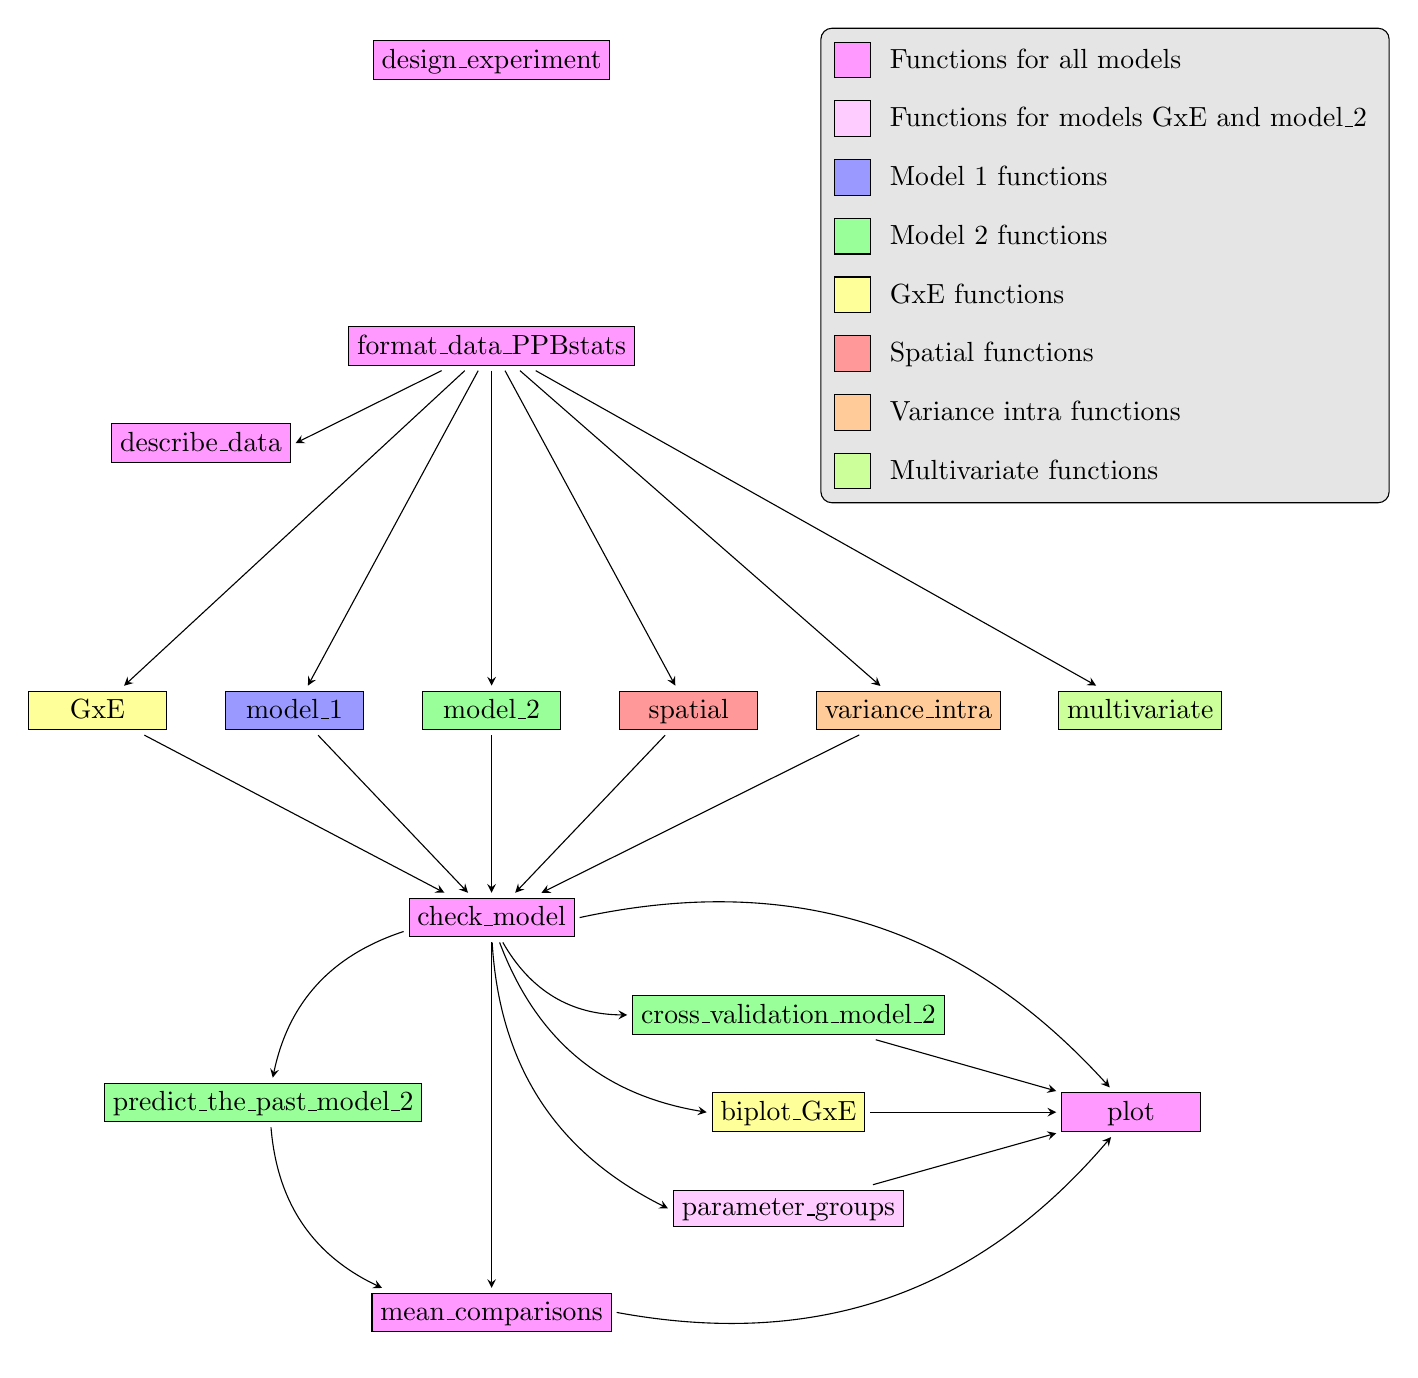
\begin{tikzpicture}

  %% nodes
  \node[several-all] (DE)                   {design\_experiment};
  
  \node[several-all] (FD) [below=3cm of DE]                {format\_data\_PPBstats};

  \node[several-all] (DD) [below left=of FD]     {describe\_data};
  
  \node[m2]   (M2)  [below=4cm of FD]        {model\_2};
  \node[m1]   (M1)  [left=of M2]   {model\_1};
  \node[gxe]  (GxE) [left=of M1]  {GxE};
  \node[sp]  (SP) [right=of M2]  {spatial};
  \node[vi]  (VI) [right=of SP]  {variance\_intra};
  \node[ma]  (MA) [right=of VI]  {multivariate};
  
  \node[several-all] (CM) [below=2cm of M2]     {check\_model};
  
  \node[virtual] (belowCM) [below=of CM] {};

  \node[m2] (PPM2)  [below left=of belowCM] {predict\_the\_past\_model\_2};
  
  \node[m2]       (CVM2)  [below right=of CM] {cross\_validation\_model\_2};
  \node[gxe]      (BGxE)  [below=of CVM2]     {biplot\_GxE};
  \node[several-gxe-m2]  (PG)    [below=of BGxE]     {parameter\_groups};
  
  \node[several-all] (MC) [below=of CM, yshift=-25ex] {mean\_comparisons};
  
  \node[several-all] (P) [right=of BGxE, xshift=5em] {plot};
  
  
  %% arrows
  % \draw node[vertex] (Joint) at (1,0) {};
  \draw (FD) to (DD.east);
  \draw (FD) to (M1);
  \draw (FD) to (M2);
  \draw (FD) to (GxE);
  \draw (FD) to (SP);
  \draw (FD) to (VI);
  \draw (FD) to (MA);
  
  \draw (M1) to (CM);
  \draw (M2) to (CM);
  \draw (GxE) to (CM);
  \draw (SP) to (CM);
  \draw (VI) to (CM);
    
  \draw (CM) to [bend right] (PPM2);
  \draw (CM) to (MC);
  \draw (CM) to [bend right] (CVM2.west);
  \draw (CM) to [bend right] (BGxE.west);
  \draw (CM) to [bend right] (PG.west);
  
  \draw (PPM2) to [bend right] (MC);
  
  \draw (CM.east) to [bend left] (P);
  \draw (CVM2) to (P);
  \draw (BGxE) to (P);
  \draw (PG) to (P);
  \draw (MC.east) to [bend right] (P);
  
  %% legend
  \node[several-all,legendkey]  (LS)  [right=of DE, xshift=6em] {};
  \node[right,legendtext] (LStext) at (LS.east) {Functions for all models};

  \node[several-gxe-m2,legendkey]  (LS2)  [below=of LS, yshift=3ex] {};
  \node[right,legendtext] (LS2text) at (LS2.east) {Functions for models GxE and model\_2};

  \node[m1,legendkey]  (LM1)  [below=of LS2,yshift=3ex] {};
  \node[right,legendtext] (LM1text) at (LM1.east) {Model 1 functions};

  \node[m2,legendkey]  (LM2)  [below=of LM1,yshift=3ex] {};
  \node[right,legendtext] (LM2text) at (LM2.east) {Model 2 functions};

  \node[gxe,legendkey]  (LGxE)  [below=of LM2,yshift=3ex] {};
  \node[right,legendtext] (LGxEtext) at (LGxE.east) {GxE functions};
  
  \node[sp,legendkey]  (LSP)  [below=of LGxE,yshift=3ex] {};
  \node[right,legendtext] (LSPtext) at (LSP.east) {Spatial functions};

  \node[vi,legendkey]  (LVI)  [below=of LSP,yshift=3ex] {};
  \node[right,legendtext] (LVItext) at (LVI.east) {Variance intra functions};

  \node[ma,legendkey]  (LMA)  [below=of LVI,yshift=3ex] {};
  \node[right,legendtext] (LMAtext) at (LMA.east) {Multivariate functions};

  %% legend bounding box
  \begin{pgfonlayer}{background}
    \node[
      fill=black!10,
      rounded corners,
      fit = (LS) (LMA) (LS2text)
    ] {};
  \end{pgfonlayer}


\end{tikzpicture}

% \end{document}